% general format definition
\documentclass[a4paper, 11pt]{article}
\usepackage[margin=.9in]{geometry}
\usepackage[utf8]{inputenc}
\usepackage[T1]{fontenc}
\usepackage[english]{babel}

% extra packages
\usepackage{hyperref}
\usepackage{listings}
\usepackage{color}
\usepackage{amssymb}
\usepackage{amsmath}
\usepackage{mathtools}
\usepackage{microtype}
\usepackage{stmaryrd}
\usepackage{tikz}
\usepackage{booktabs}
\usepackage{stmaryrd}
\usepackage{enumitem}

% Abbildungen
\usepackage{makecell}
\usepackage{multirow}
\usepackage{colortbl}
\usepackage{hhline}
\usepackage{vcell}
\usepackage{graphicx}
\usepackage{multicol}

% special math symbols
\newcommand{\R}{\ensuremath{\mathbb{R}}}
\newcommand{\N}{\ensuremath{\mathbb{N}}}
\newcommand{\Z}{\ensuremath{\mathbb{Z}}}
\newcommand{\Q}{\ensuremath{\mathbb{Q}}}

% Fraktur für Strukturen
\newcommand{\A}{\ensuremath{\mathfrak A}}
\newcommand{\B}{\ensuremath{\mathfrak B}}
\newcommand{\C}{\ensuremath{\mathfrak C}}
\newcommand{\I}{\ensuremath{\mathfrak I}}

% logical operators
\newcommand{\xor}{\ensuremath{\oplus}} %exklusives oder
\newcommand{\impl}{\ensuremath{\rightarrow}} %logische Implikation

% nicer symbols
\renewcommand{\phi}{\varphi}
\renewcommand{\theta}{\vartheta}
\renewcommand{\epsilon}{\varepsilon}

% Syntax highlighting
\definecolor{commentsColor}{rgb}{0.497495, 0.497587, 0.497464}
\definecolor{keywordsColor}{rgb}{0.000000, 0.000000, 0.635294}
\definecolor{stringColor}{rgb}{0.558215, 0.000000, 0.135316}
\definecolor{brightlavender}{rgb}{0.75, 0.58, 0.89}
\definecolor{brilliantrose}{rgb}{1.0, 0.33, 0.64}
\definecolor{canaryyellow}{rgb}{1.0, 0.94, 0.0}
\definecolor{cyan}{rgb}{0.0, 1.0, 1.0}
\definecolor{fulvous}{rgb}{0.86, 0.52, 0.0}
\definecolor{olive}{rgb}{0.5, 0.5, 0.0}
\lstset{
  backgroundcolor=\color{white},                        % choose the background color; you must add \usepackage{color} or \usepackage{xcolor}
  basicstyle=\footnotesize,                             % the size of the fonts that are used for the code
  breakatwhitespace=false,                              % sets if automatic breaks should only happen at whitespace
  breaklines=true,                                      % sets automatic line breaking
  captionpos=b,                                         % sets the caption-position to bottom
  commentstyle=\color{commentsColor}\textit,            % comment style
  deletekeywords={},                                    % if you want to delete keywords from the given language
  escapeinside={\%*}{*)},                               % if you want to add LaTeX within your code
  extendedchars=true,                                   % lets you use non-ASCII characters; for 8-bits encodings only, does not work with UTF-8
  frame=tb,	                   	                        % adds a frame around the code
  keepspaces=true,                                      % keeps spaces in text, useful for keeping indentation of code (possibly needs columns=flexible)
  keywordstyle=\color{keywordsColor}\bfseries,          % keyword style
  otherkeywords={True,False,true,false,null,None,NULL}, % if you want to add more keywords to the set
  numbers=left,                                         % where to put the line-numbers; possible values are (none, left, right)
  numbersep=5pt,                                        % how far the line-numbers are from the code
  numberstyle=\tiny\color{commentsColor},               % the style that is used for the line-numbers
  rulecolor=\color{black},                              % if not set, the frame-color may be changed on line-breaks within not-black text (e.g. comments (green here))
  showspaces=false,                                     % show spaces everywhere adding particular underscores; it overrides 'showstringspaces'
  showstringspaces=false,                               % underline spaces within strings only
  showtabs=false,                                       % show tabs within strings adding particular underscores
  stepnumber=1,                                         % the step between two line-numbers. If it's 1, each line will be numbered
  stringstyle=\color{stringColor},                      % string literal style
  tabsize=2,	                                          % sets default tabsize to 2 spaces
  title=\lstname,                                       % show the filename of files included with \lstinputlisting; also try caption instead of title
  columns=fixed,                                        % Using fixed column width (for e.g. nice alignment)
}



% TIKZ settings
\usetikzlibrary{arrows,calc,trees}
\usetikzlibrary{arrows,positioning, calc,lindenmayersystems,decorations.pathmorphing,intersections}
\tikzstyle{resource}= [draw,minimum size=16pt,inner sep=0pt]
\tikzstyle{process} = [draw,minimum size=16pt,inner sep=0pt,circle]
\tikzstyle{allocated} = [->,thick,arrows={-latex}]
\tikzstyle{requested} = [<-,thick,arrows={latex-}, dashed]

\author{Thilo Metzlaff\\406247 \and Mats Frenk\\393702\and Emma van Emelen\\406008}
\title{BUS Exercise 6 \\ Group 23}
\begin{document}
      % titlepage
      \maketitle
      \newpage

      % contents
      \tableofcontents
      \newpage

      % section 0
      \section*{Introduction}
      And \texttt{A G A I N}, welcome to this document of absolute bullshittery, written in \LaTeX. This will be one of my Low-Effort documents, with low-effort answers. Why? idk, i just feel like it.
      Having absolutely no energy REALLY doesn't make it better... but i shall prevail. With the help of premade solutions by a friend, because i truly have no time or energy to even try. Humor will be limited.


      \subsection*{THE FORMAT}
      \begin{itemize}
            \item Every file will be named similar to the sections in here, so\\
            \texttt{2.1-stack\_exercise.c} is Exercise 2, section 1.
            \item Every Solution \textbf{WILL} be in this pdf, but not necessarily 
                  anything predefined by the exercise.
            \item Any explanation will be both in this PDF as well as in each file.
            \item This explanation will be in each PDF, in case someone who doesn't
                  know the format tries to correct the exercises
            \item \textbf{WARNING:} Humor may or may not be used. If you are allergic
                  to humor, that sounds like a personal problem.
            \item \textbf{WARNING:} Backing up your data is important. Although linux 
                  doesn't have the necessary shame to remove itself, unlike windows,
                  please do back up your data. And try to keep track of your periods\dots
                  they seem to be notoriously hard to find
      \end{itemize}
      \newpage

      \section{Things i can't process}
      \subsection{The infinity Square}
      \begin{table}[h!]
      \centering
      \arrayrulecolor{black}
      \scalebox{1.5}{%
      \begin{tabular}{|c|l|llll!{\color[rgb]{0,0.902,0}\vrule}llllll|} 
      \cline{1-2}\arrayrulecolor[rgb]{1,0.647,0}\cline{3-6}\arrayrulecolor{black}\cline{7-12}
      \multirow{11}{*}{\rotcell{ Process B }} & 10               & \multicolumn{4}{c!{\color[rgb]{1,0.647,0}\vrule}}{\multirow{2}{*}{   BM4}}                                                                                                                                                                    &                                                         &                        &                                                    &                                                     &                        &     \\ 
      \cline{2-2}\arrayrulecolor[rgb]{0.859,0,0.859}\cline{8-10}
                                          & 9                & \multicolumn{4}{c!{\color[rgb]{1,0.647,0}\vrule}}{}                                                                                                                                                                                           & \multicolumn{1}{l!{\color[rgb]{0.859,0,0.859}\vrule}}{} & \multicolumn{3}{c!{\color[rgb]{0.859,0,0.859}\vrule}}{BM5}                                                                        &                        &     \\ 
      \arrayrulecolor{black}\cline{2-2}\arrayrulecolor{red}\cline{4-5}\arrayrulecolor[rgb]{0.859,0,0.859}\cline{8-10}
                                          & 8                & \multicolumn{1}{l!{\color{red}\vrule}}{}                                                        & \multicolumn{2}{c!{\color{red}\vrule}}{BM2}                                       & \multicolumn{1}{l!{\color[rgb]{1,0.647,0}\vrule}}{}     &                                                         &                        &                                                    &                                                     &                        &     \\ 
      \hhline{>{\arrayrulecolor{black}}|~->{\arrayrulecolor[rgb]{1,0.647,0}}--->{\arrayrulecolor[rgb]{0,0.761,0.761}}-->{\arrayrulecolor[rgb]{0.455,0.455,0.455}}----->{\arrayrulecolor{black}}|}
                                          & \vcell{7}        & \multicolumn{1}{l!{\color{red}\vrule}}{{\cellcolor[rgb]{0.753,0.753,0.753}}}                    & \vcell{}               & \multicolumn{1}{l!{\color{red}\vrule}}{\vcell{}}         & \multicolumn{2}{c!{\color[rgb]{0,0.761,0.761}\vrule}}{\multirow{2}{*}{BM1}}                                       & \multicolumn{2}{c}{{\cellcolor[rgb]{0.455,0.455,0.455}}}                    & \multicolumn{3}{l|}{{\cellcolor[rgb]{0.455,0.455,0.455}}\vcell{}}                  \\[-\rowheight]
                                          & \printcellmiddle & \multicolumn{1}{l!{\color{red}\vrule}}{{\cellcolor[rgb]{0.753,0.753,0.753}}}                    & \printcellmiddle       & \multicolumn{1}{l!{\color{red}\vrule}}{\printcellmiddle} & \multicolumn{2}{c!{\color[rgb]{0,0.761,0.761}\vrule}}{}                                                           & \multicolumn{2}{c}{{\cellcolor[rgb]{0.455,0.455,0.455}}}                    & \multicolumn{3}{l|}{{\cellcolor[rgb]{0.455,0.455,0.455}}\printcellmiddle}          \\ 
      \hhline{|~->{\arrayrulecolor[rgb]{0.753,0.753,0.753}}-~~~~>{\arrayrulecolor[rgb]{0.455,0.455,0.455}}-->{\arrayrulecolor{black}}---|}
                                          & 6                & \multicolumn{1}{l!{\color{red}\vrule}}{\multirow{-2}{*}{{\cellcolor[rgb]{0.753,0.753,0.753}}u}} &                        & \multicolumn{1}{l!{\color{red}\vrule}}{}                 & \multicolumn{2}{c!{\color[rgb]{0,0.761,0.761}\vrule}}{}                                                           & \multicolumn{2}{c}{\multirow{-2}{*}{{\cellcolor[rgb]{0.455,0.455,0.455}}i}} & \multicolumn{3}{l|}{BM6}                                                           \\ 
      \cline{2-2}\arrayrulecolor{red}\cline{4-5}\arrayrulecolor[rgb]{0,0.902,0}\cline{7-9}
                                          & 5                &                                                                                                 &                        & \multicolumn{1}{l!{\color[rgb]{0,0.761,0.761}\vrule}}{}  &                                                         & \multicolumn{1}{l!{\color[rgb]{0,0.761,0.761}\vrule}}{} &                        & \multicolumn{1}{l|}{}                              & \multicolumn{1}{l!{\color[rgb]{0,0.902,0}\vrule}}{} &                        &     \\ 
      \hhline{>{\arrayrulecolor{black}}|~-~~~>{\arrayrulecolor[rgb]{0,0.761,0.761}}--~~~~~>{\arrayrulecolor{black}}|}
                                          & 4                &                                                                                                 &                        &                                                          & {\cellcolor[rgb]{0.753,0.753,0.753}}                    &                                                         & \multicolumn{2}{l|}{BM3}                                                    & \multicolumn{1}{l!{\color[rgb]{0,0.902,0}\vrule}}{} &                        &     \\ 
      \hhline{|~-~~~>{\arrayrulecolor[rgb]{0.753,0.753,0.753}}-~~~>{\arrayrulecolor{black}}---|}
                                          & 3                &                                                                                                 &                        &                                                          & \multirow{-2}{*}{{\cellcolor[rgb]{0.753,0.753,0.753}}u} &                                                         &                        &                                                    & \multicolumn{1}{l!{\color[rgb]{0,0.902,0}\vrule}}{} &                        &     \\ 
      \cline{2-2}\arrayrulecolor[rgb]{0,0.902,0}\cline{7-10}
                                          & 2                &                                                                                                 &                        &                                                          & \multicolumn{1}{l}{}                                    &                                                         &                        &                                                    &                                                     &                        &     \\ 
      \arrayrulecolor{black}\cline{2-2}
                                          & 1                &                                                                                                 &                        &                                                          & \multicolumn{1}{l}{}                                    &                                                         &                        &                                                    &                                                     &                        &     \\ 
      \cline{2-12}
                                          &                  & \multicolumn{1}{l|}{1}                                                                          & \multicolumn{1}{l|}{2} & \multicolumn{1}{l|}{3}                                   & \multicolumn{1}{l|}{4}                                  & \multicolumn{1}{l|}{5}                                  & \multicolumn{1}{l|}{6} & \multicolumn{1}{l|}{7}                             & \multicolumn{1}{l|}{8}                              & \multicolumn{1}{l|}{9} & 10  \\ 
      \hline
      \multicolumn{1}{|l|}{}                  & \multicolumn{11}{c|}{          Process A}                                                                                                                                                                                                                                                                                                                                                                                                                                                     \\
      \hline
      \end{tabular}}
      \end{table}
      u = unsafe; n = impossible

      \subsection{The no effort name for the no effort answer}
      \begin{itemize}[leftmargin=\parindent+.28in]
            \item[$(6,4)$ -] unmöglich
            \item[$(4,3)$ -] unsicher
            \item[$(9,8)$ -] sicher
            \item[$(6,6)$ -] unmöglich
      \end{itemize}
      \newpage
      
      \subsection{Pathfinding and walking around processes}
      \begin{table}[h]
            \centering
            \arrayrulecolor{black}
            \scalebox{1.5}{%
            \begin{tabular}{|c|l|lll!{\color[rgb]{1,0.361,0.361}\vrule}!{\color[rgb]{1,0.361,0.361}\vrule}l!{\color[rgb]{0,0.902,0}\vrule}llll!{\color[rgb]{0,0.902,0}\vrule}ll|} 
            \hhline{|-->{\arrayrulecolor[rgb]{1,0.647,0}}---->{\arrayrulecolor{black}}---->{\arrayrulecolor[rgb]{1,0.361,0.361}}|t:==>{\arrayrulecolor{black}}|}
            \multirow{11}{*}{\rotcell{ Prozess B }} & 10               & \multicolumn{4}{c!{\color[rgb]{1,0.647,0}\vrule}}{\multirow{2}{*}{BM4}}                                                                                                                                     &                                                                                            &                        &                                                    & \multicolumn{1}{l!{\color[rgb]{1,0.361,0.361}\vrule}!{\color[rgb]{1,0.361,0.361}\vrule}}{} &                        &     \\ 
            \cline{2-2}\arrayrulecolor[rgb]{0.859,0,0.859}\cline{8-10}
                                                    & 9                & \multicolumn{4}{c!{\color[rgb]{1,0.647,0}\vrule}}{}                                                                                                                                                         & \multicolumn{1}{l!{\color[rgb]{0.859,0,0.859}\vrule}}{}                                    & \multicolumn{3}{c!{\color[rgb]{1,0.361,0.361}\vrule}!{\color[rgb]{1,0.361,0.361}\vrule}}{BM5}                                                                            &                        &     \\ 
            \hhline{>{\arrayrulecolor{black}}|~-~>{\arrayrulecolor{red}}--~~>{\arrayrulecolor[rgb]{1,0.361,0.361}}|t:===:b|~~>{\arrayrulecolor{black}}|}
                                                    & 8                & \multicolumn{1}{l!{\color{red}\vrule}}{}                                                        & \multicolumn{2}{c!{\color{red}\vrule}}{BM2}     & \multicolumn{1}{l!{\color[rgb]{1,0.647,0}\vrule}}{}     & \multicolumn{1}{l!{\color[rgb]{1,0.361,0.361}\vrule}!{\color[rgb]{1,0.361,0.361}\vrule}}{} &                        &                                                    & \multicolumn{1}{l}{}                                                                       &                        &     \\ 
            \hhline{|~->{\arrayrulecolor[rgb]{1,0.647,0}}--->{\arrayrulecolor[rgb]{1,0.361,0.361}}|t:==>{\arrayrulecolor[rgb]{0,0.761,0.761}}:b|>{\arrayrulecolor[rgb]{0.455,0.455,0.455}\doublerulesepcolor[rgb]{0.455,0.455,0.455}}=====>{\arrayrulecolor{black}}|}\doublerulesepcolor{white}
                                                    & \vcell{7}        & \multicolumn{1}{l!{\color{red}\vrule}}{{\cellcolor[rgb]{0.753,0.753,0.753}}}                    & \vcell{}               & \vcell{}               & \multicolumn{2}{c!{\color[rgb]{0,0.761,0.761}\vrule}}{\multirow{2}{*}{BM1}}                                                                          & \multicolumn{2}{c}{{\cellcolor[rgb]{0.455,0.455,0.455}}}                    & \multicolumn{3}{l|}{{\cellcolor[rgb]{0.455,0.455,0.455}}\vcell{}}                                                         \\[-\rowheight]
                                                    & \printcellmiddle & \multicolumn{1}{l!{\color{red}\vrule}}{{\cellcolor[rgb]{0.753,0.753,0.753}}}                    & \printcellmiddle       & \printcellmiddle       & \multicolumn{2}{c!{\color[rgb]{0,0.761,0.761}\vrule}}{}                                                                                              & \multicolumn{2}{c}{{\cellcolor[rgb]{0.455,0.455,0.455}}}                    & \multicolumn{3}{l|}{{\cellcolor[rgb]{0.455,0.455,0.455}}\printcellmiddle}                                                 \\ 
            \hhline{|~->{\arrayrulecolor[rgb]{0.753,0.753,0.753}}-~~>{\arrayrulecolor[rgb]{1,0.361,0.361}}||~~>{\arrayrulecolor[rgb]{0.455,0.455,0.455}}-->{\arrayrulecolor{black}}---|}
                                                    & 6                & \multicolumn{1}{l!{\color{red}\vrule}}{\multirow{-2}{*}{{\cellcolor[rgb]{0.753,0.753,0.753}}u}} &                        &                        & \multicolumn{2}{c!{\color[rgb]{0,0.761,0.761}\vrule}}{}                                                                                              & \multicolumn{2}{c}{\multirow{-2}{*}{{\cellcolor[rgb]{0.455,0.455,0.455}}n}} & \multicolumn{3}{l|}{BM6}                                                                                                  \\ 
            \cline{2-2}\arrayrulecolor{red}\cline{4-5}\arrayrulecolor[rgb]{0,0.902,0}\cline{7-9}
                                                    & 5                &                                                                                                 &                        &                        &                                                         & \multicolumn{1}{l!{\color[rgb]{0,0.761,0.761}\vrule}}{}                                    &                        & \multicolumn{1}{l|}{}                              &                                                                                            &                        &     \\ 
            \hhline{>{\arrayrulecolor{black}}|~-~~~>{\arrayrulecolor[rgb]{1,0.361,0.361}}||>{\arrayrulecolor[rgb]{0,0.761,0.761}}--~~~~~>{\arrayrulecolor{black}}|}
                                                    & 4                &                                                                                                 &                        &                        & {\cellcolor[rgb]{0.753,0.753,0.753}}                    &                                                                                            & \multicolumn{2}{l|}{BM3}                                                    &                                                                                            &                        &     \\ 
            \hhline{|~-~~~>{\arrayrulecolor[rgb]{1,0.361,0.361}}||>{\arrayrulecolor[rgb]{0.753,0.753,0.753}}-~~~>{\arrayrulecolor{black}}---|}
                                                    & 3                &                                                                                                 &                        &                        & \multirow{-2}{*}{{\cellcolor[rgb]{0.753,0.753,0.753}}u} &                                                                                            &                        &                                                    &                                                                                            &                        &     \\ 
            \cline{2-2}\arrayrulecolor[rgb]{0,0.902,0}\cline{7-10}
                                                    & 2                &                                                                                                 &                        &                        & \multicolumn{1}{l}{}                                    &                                                                                            &                        &                                                    & \multicolumn{1}{l}{}                                                                       &                        &     \\ 
            \arrayrulecolor{black}\cline{2-2}
                                                    & 1                &                                                                                                 &                        &                        & \multicolumn{1}{l}{}                                    &                                                                                            &                        &                                                    & \multicolumn{1}{l}{}                                                                       &                        &     \\ 
                                                    \hhline{|~->{\arrayrulecolor[rgb]{1,0.361,0.361}}===>{\arrayrulecolor{black}}:b|-------|}
                                                    &                  & \multicolumn{1}{l|}{1}                                                                          & \multicolumn{1}{l|}{2} & \multicolumn{1}{l|}{3} & \multicolumn{1}{l|}{4}                                  & \multicolumn{1}{l|}{5}                                                                     & \multicolumn{1}{l|}{6} & \multicolumn{1}{l|}{7}                             & \multicolumn{1}{l|}{8}                                                                     & \multicolumn{1}{l|}{9} & 10  \\ 
            \hline
            \multicolumn{1}{|l|}{}                  & \multicolumn{11}{c|}{Prozess A}                                                                                                                                                                                                                                                                                                                                                                                                                                                                                                       \\
            \hline
            \end{tabular}}
      \end{table}
      \begin{center}
            Schedule: AAABBBBBBBAABAAABBAA
      \end{center}
      \newpage

      \section{Banker Algorithm}
      
        \subsection{Dreadlock prevention}
        \label{sec:bank_alg}
        \begin{enumerate}
            \item $P_1$ is unmarked
            \begin{enumerate}
                \item[1.] Test: $Q_1^{max}(k) = (2,4,2) \leq V(k) = (3,3,4) \rightarrow nicht$ 
            \end{enumerate}
            \item $P_2$ is unmarked
            \begin{enumerate}
                \item[1.] test: $Q_2^{max}(k) = (4,1,1) \leq V(k) = (3,3,4) \rightarrow nicht$ 
            \end{enumerate}
            \item $P_3$ is unmarked
            \begin{enumerate}
                \item[1.] test: $Q_3^{max}(k) = (2,1,4) \leq V(k) = (3,3,4)$
                \item[2.] $V(k) = V(k) + H_3(k) = (5,3,4)$
                \item[3.] Markiere $P_3$ 
            \end{enumerate}
            \item $P_1$ is unmarked
            \begin{enumerate}
                \item[1.] test: $Q_1^{max}(k) = (2,4,2) \leq V(k) = (5,3,4)$
                \item[2.] $V(k) = V(k) + H_2(k) = (6,5,4)$
                \item[3.] Markiere $P_1$ 
            \end{enumerate}
            \item $P_2$ is unmarked
            \begin{enumerate}
                \item[1.] test: $Q_2^{max}(k) = (4,1,1) \leq V(k) = (6,5,4)$
                \item[2.] $V(k) = V(k) + H_2(k) = (6,6,4)$
                \item[3.] Markiere $P_2$ 
            \end{enumerate}
      \end{enumerate}
      $\Rightarrow$ All processes are marked, therefore the state is safe.
      \newpage

      \subsection{Evil Dreadlocks}
      \begin{enumerate}
            \item[1].)
            \begin{enumerate}
                \item[1.1] $Q_1^{akt}(k) = (0,0,1) \leq (3,3,4) = V(k)$
                \item[1.2] Trying:
                \begin{align*}
                    &V(k) = V(k) - Q_1^{akt}(k) = (3,3,3) \\
                    &H_1(k) = H_1(k) +Q_1^{akt}(k) = (1,2,1) \\
                    &Q_1^{max}(k) = Q_1^{max}(k) - Q_1^{akt}(k) = (2,4,1) 
                \end{align*} 
                \item[1.3] Security test: \\
                 $P_3$ cannot be executed anymore: $Q_3^{max}(k) \mbox{ } \lneq V(k) = (3,3,3)$ \\
                 $P_2$ cannot be executed anymore: $Q_2^{max}(k) \mbox{ } \lneq V(k) = (3,3,3)$ \\
                 $P_1$ cannot be executed anymore: $Q_1^{max}(k) \mbox{ } \lneq V(k) = (3,3,3)$ \\\\
                 $\Rightarrow$ unsafe state
            \end{enumerate}
            \item[2].)
            \begin{enumerate}
                \item[2.1] $Q_1^{akt}(k) = (0,4,0) \mbox{ } \lneq (3,3,4) = V(k)$
                \begin{enumerate}
                    \item[]  $Q_1^{akt}$ cannot be executed $\Rightarrow$ unsafe/deadlock
                \end{enumerate}
            \end{enumerate}
            \item[3].) 
            \begin{enumerate}
                \item[3.1] $Q_2^{akt}(k) = (1,0,0) \leq (3,3,4) = V(k)$
                \item[3.2] Trying: 
                \begin{align*}
                    &V(k) = V(k) - Q_2^{akt}(k) = (2,3,4) \\
                    &H_2(k) = H_2(k) +Q_2^{akt}(k) = (1,1,0) \\
                    &Q_2^{max}(k) = Q_2^{max}(k) - Q_2^{akt}(k) = (3,1,1) 
                \end{align*}
                \item[3.3] Security test: \\
                $P_3$ cannot be executed anymore:\\ $Q_3^{max}(k) \mbox{ } \lneq V(k) = (2,3,4) \rightarrow V(k) = (4,3,4)$ \\
                $P_2$ cannot be executed anymore: \\ $Q_2^{max}(k) \mbox{ } \lneq V(k) = (4,3,4) \rightarrow V(k) = (5,5,4)$ \\
                $P_1$ cannot be executed anymore: \\ $Q_1^{max}(k) \mbox{ } \lneq V(k) = (5,5,4) \rightarrow V(k) = (6,6,4)$ \\
                $\Rightarrow$ safe state
            \end{enumerate} 
        \end{enumerate}

        \subsection{}
        
        Assumption $P_1$ can run $BM_2$ at most twice at time $k$. \\
        Because $V(k) - (0,2,0) = (3,1,4)$ \\
        And $Q_3^{max} \leq (3,1,4) \Rightarrow$ Banker algoritm is executable like in \textit{\texttt{\autoref{sec:bank_alg}}}. \\
        And $V(k) - (0,3,0) = (3,0,4)$ \\
        And $Q_3^{max} \mbox{ } !\leq (3,0,4) \Rightarrow$ Banker algoritm is not executable like in \textit{\texttt{\autoref{sec:bank_alg}}}
        \newpage

        \section{Resource Allocation Graphs}
        \subsection{The fun RAG}
        \begin{table}[h!]
            \centering
            \begin{tabular}{|l||l|l|l|l|l|l|l|l|l|l|} 
                  \hline
                  \multicolumn{1}{|l|}{} & 1  & 2    & 3    & 4     & 5    & 6     & 7    & 8    & 9    & 10    \\ 
                  \hhline{|=:t:==========|}
                  $P_1$               & A+ & A, c & A, c & A, C+ & A, C & A-, C & C, b & C, b & C, b & C, b  \\ 
                  \hline
                  $P_2$               &    & a    & a    & a     & a    & a     & A+   & A    & A, c & A, c  \\ 
                  \hline
                  $P_3$               & C+ & C    & C-   & B+    & B, a & B, a  & B, a & B,a  & B, a & B,a   \\
                  \hline
            \end{tabular}
      \end{table}

      \subsection{Graphs to the people}
      \subsubsection{Resource Allocation Graph}
      \begin{figure}[h!]
            \centering
            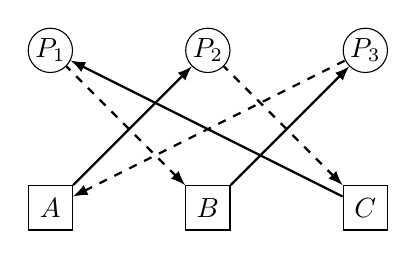
\begin{tikzpicture}[scale=2]
                  \node (r1)[resource] at (0,1) {$A$};
                  \node (r2)[resource] at (1,1) {$B$};
                  \node (r3)[resource] at (2,1) {$C$};
                  \node (p1)[process]  at (0,2) {$P_1$};   
                  \node (p2)[process]  at (1,2) {$P_2$};
                  \node (p3)[process]  at (2,2) {$P_3$};
                  
                  \draw[allocated] (r3) -- (p1);
                  \draw[requested] (r2) -- (p1);
                  \draw[allocated] (r1) -- (p2);
                  \draw[requested] (r3) -- (p2);
                  \draw[allocated] (r2) -- (p3);
                  \draw[requested] (r1) -- (p3);
            \end{tikzpicture}
      \end{figure}
      \begin{center}
            \textit{Dotted lines are requests, whereas solid lines are allocations.}
      \end{center}
      
      \subsubsection{LEGEN- ... Wait-For it... }
      \begin{multicols}{3}
            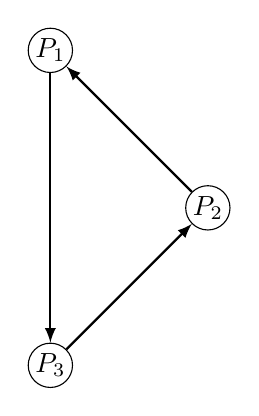
\begin{tikzpicture}[scale=2]
                  \node (p1)[process]  at (0,0) {$P_3$};   
                  \node (p2)[process]  at (1,1) {$P_2$};
                  \node (p3)[process]  at (0,2) {$P_1$};
            
                  \draw[allocated] (p3) -- (p1) ;
                  \draw[allocated] (p2) -- (p3) ;
                  \draw[allocated] (p1) -- (p2) ;
            \end{tikzpicture}
            \begin{itemize}
                  \item circular wait: see "Wait for graph"
                  \item Non-Preemption: as defined by Exercise
                  \item Hold and wait: as defined by Exerciseg
                  \item Exclusive Use: as defined by Exercise
                  \item[$\Rightarrow$] therefore we have a deadlock.
            \end{itemize}
      \end{multicols}
      \newpage

      \subsection{Resource unavailable.}
      \begin{table}[h!]
            \centering
            \begin{tabular}{|l||l|l|l|l|l|l|l|l|l|l|} 
                  \hline
                  \multicolumn{1}{|l|}{} & 1  & 2    & 3    & 4     & 5    & 6     & 7    & 8    & 9    & 10    \\ 
                  \hhline{|=:t:==========|}
                  $P_1$               & A+ & A, c & A, c & A, C+ & A, C & A-, C & C, b & C, b & C, b & C, b  \\ 
                  \hline
                  $P_2$               &    & a    & a    & a     & a    & a     & a   & a    & a & A+  \\ 
                  \hline
                  $P_3$               & C+ & C    & C-   & B+    & B, a & B, a  & B, A+ & B,A  & B, A- & B-   \\
                  \hline
            \end{tabular}
      \end{table}
      \subsubsection{RAG time}
      \begin{figure}[h!]
            \centering
            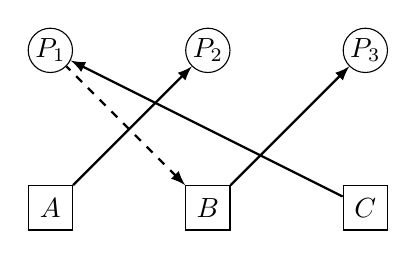
\begin{tikzpicture}[scale=2]
                  \node (r1)[resource] at (0,1) {$A$};
                  \node (r2)[resource] at (1,1) {$B$};
                  \node (r3)[resource] at (2,1) {$C$};
                  \node (p1)[process]  at (0,2) {$P_1$};   
                  \node (p2)[process]  at (1,2) {$P_2$};
                  \node (p3)[process]  at (2,2) {$P_3$};
            
                  \draw[allocated] (r3) -- (p1);
                  \draw[requested] (r2) -- (p1);
                  \draw[allocated] (r1) -- (p2);
                  \draw[allocated] (r2) -- (p3);
            \end{tikzpicture}
      \end{figure}
      \begin{center}
            \textit{Dotted lines are requests, whereas solid lines are allocations.}
      \end{center}
      \subsubsection{wait for it... -DARY}
      \begin{multicols}{3}
            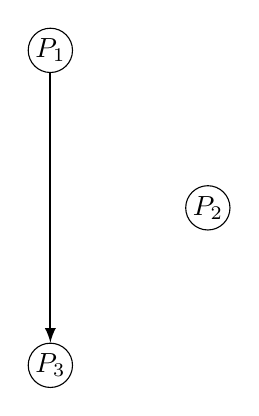
\begin{tikzpicture}[scale=2]
                \node (p1)[process]  at (0,0) {$P_3$};   
                \node (p2)[process]  at (1,1) {$P_2$};
                \node (p3)[process]  at (0,2) {$P_1$};
            
                \draw[allocated] (p3) -- (p1) ;
            \end{tikzpicture}
            \begin{itemize}
                \item circular wait: doesn't exist, see "Wait for graph"
                \item[] $\Rightarrow$ therefore we have a deadlock.
            \end{itemize}
      \end{multicols}

      \subsection{The end}
      Due to the fact that $P_3$ terminates in step 10, $B$ is free which lets all processs Terminate. Therefore $P_1$ doesn't have to wait for $B$ and can rest in piece, after finishing. Now $P_3$ can run without interruptions.   
\end{document}